\chapter{Introduction to SLAM}
SLAM stays for Simultaneous Localization And Mapping. It is a particular field of robotics/AI that aims to guess the actual state of the world, given some data acquired by the robot.
Data could be robot poses, camera images associated to these poses, sonar acquisitions and many more.
Needless to say, these data are usually affected by noise, meaning that solving SLAM problems usually involves a certain level of uncertainties.

\section{Graph model}
There is a quite suitable way to represent our knowledge about the world, that is using a graph.
Nodes are either robot poses or landmarks.
Edges are constraints between nodes.
In this way, you can imagine the graph as a lot of nodes, with springs that ``pull and push'' these nodes.
The solution that minimizes the overall ``force'' is the one that we take as guess about the world.

\begin{figure}[htbp]
  \centering
    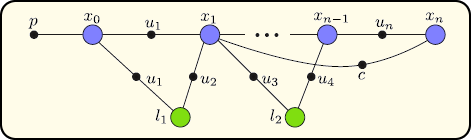
\includegraphics[width=0.5\textwidth]{images/graph.png}
  \caption{Data representation graph. Blue nodes are poses, green ones are landmarks.}
\end{figure}

